
\documentclass[../../header.tex]{subfiles}

\begin{document}
%This is Question from Cheng 3-28
\textbf{Goal:} Dielectric lenses can be used to collimate electromagnetic fields. In the diagram below, the left surface of the lens is that of a circular cylinder, and the right surface is a plane. If $\vec{E}_1$ at point $P(r_o, 45^\circ, z)$ is region $1$ is $5\vec{a}_r - 3\vec{a}_\phi$, what must be the dielectric constant of the lens in order that $\vec{E}_3$ in region $3$ is parallel to the $x$-axis?
\begin{center}
	\includegraphics[width=0.2\textwidth]{\wpath Q3-28.pdf}
\end{center}
\textbf{Steps:} 
\begin{enumerate}
\item Draw the electric fields vectors at the point $P$.

\solution{
\begin{center}
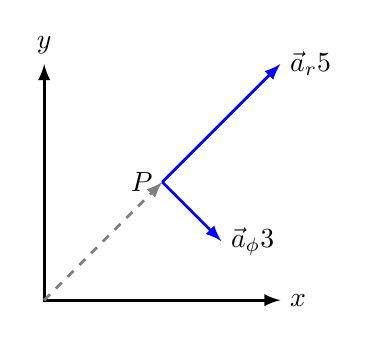
\begin{tikzpicture}[scale=1.5,>=latex]
\draw [<->,line width=1pt] (2,0) -| (0,2);
\node [right] at (2,0) {$x$};
\node [above] at (0,2) {$y$};
\draw [dashed,gray,->,line width=1pt] (0,0) -- (1,1);
\node [left] at (1,1) {$P$};
\draw [blue,->, line width=1pt] (1,1) -- +(0.5,-0.5);
\node [right] at (1.5,0.5) {$\vec{a}_\phi 3$};
\draw [blue,->, line width=1pt] (1,1) -- +(1,1);
\node [right] at (2,2) {$\vec{a}_r 5$};
\end{tikzpicture}
\end{center}}

\item What are the boundary conditions of the E-fields across a dielectric interface?

\solution{
The tangential electric fields is continuous across the boundary. The normal electric fields are scaled by the ratio of the dielectric constant on either side.
\begin{equation*}
\frac{E_{\mathrm{n}2}}{E_{\mathrm{n}1}} = \frac{\varepsilon_1}{\varepsilon_2}
\end{equation*}}

\item Compute the dielectric constant of the lens.

\solution{
We simply scale $5\vec{a}_r$ (the normal vector) such that its $y$-component is the same as the $y$-component of $3\vec{a}_\phi$. Hence dielectric constant needs to be $5/3$.}
\end{enumerate}
\answer{$\varepsilon_r$\,=\,5/3}
\end{document}




































